\section{Adversarial Attack}  
Both adversarial attacks and backdoor attacks are
techniques used to modify benign testing samples in order
to make models misbehave during the inference process.
While adversarial perturbations are sample-agnostic in
universal adversarial attacks, these attacks can appear
similar to backdoor attacks. Consequently, researchers
who are unfamiliar with backdoor attacks may question
their significance, as these attacks require additional
controls on the training process to some extent. However,
despite certain similarities, these attacks have essential
differences.

Firstly, adversarial attackers need to control the
inference process to a certain degree but not the training
process of models. They must query the model results
or even gradients multiple times to generate adversarial
perturbations by optimization, given a fixed targeted
model. On the other hand, backdoor attackers require
modifying certain training stages, such as data collection
and model training, without any additional requirements
in the inference process. Secondly, from the perspective
of attacked samples, backdoor attackers use known,
non-optimized perturbations, whereas adversarial attackers
require obtaining them through the optimization process
based on the model output. This optimization in
adversarial attacks requires multiple queries, making them unable
to be real-time in many cases. Finally, the mechanisms
of these attacks are fundamentally different. Adversarial
vulnerability results from the differences in behaviors of
models and humans, while backdoor attackers exploit the
excessive learning ability of deep neural networks (DNNs)
to establish a latent connection between trigger patterns
and target labels.  

In federated learning, because the data is not shared
among participants, attackers can use this to generate
adversarial samples locally, then inject them into the data
sets of participants, and train the model with the data of
other participants during the training process.
So, how should attacks targeting federated learning be
designed? In centralized learning, FGSM [99] is initially
used to generate adversarial examples. Let $\theta$ be the parameters of a model, $x$ the input to the model,
$eta$ the perturbation to original input and $||\eta||_\infty \le \epsilon$,
$y$ the targets associated with $x$ (for machine learning tasks that have targets)
and $J(\theta, x, y)$ be the cost used to train the neural network.
We can linearize the cost function around the current value of $\theta$,
obtaining an optimal max-norm constrained pertubation of:
\begin{equation}
    \eta = \epsilon sign(\nabla_x J(\theta,x,y))
\end{equation}

In federated learning, attackers can use FGSM locally to generate
adversarial samples and then inject them into the datasets of some participants
to affect the performance of the entire model.

In federated learning, attackers can use FGSM locally
to generate adversarial samples and then inject them into
the datasets of some participants to affect the performance
of the entire model. PGD [100] is a more powerful adversarial sample
generation method, which generates adversarial samples
by iteratively perturbing the input. Specifically, PGD
first randomly generates an initial disturbance $\delta_0$,
and then iteratively updates the disturbance $\delta_t$, to meet the constraint,
that is, $|\delta_t|_{\infty} \leq \epsilon_{\text{max}}$,
where $\epsilon_{\text{max}}$is the maximum value of the disturbance.
After each update, PGD also projects the disturbance
$\delta_t$ back into the constraint space to ensure that it meets the
constraint conditions.
Specifically, the update formula for PGD is as follows:
\begin{equation}
    x^{t+1} = \text{Clip}(x + \text{sign}(\nabla_x L(\theta,x',y)) \cdot \epsilon{\text{max}}, x - \epsilon_{\text{max}}, x + \epsilon_{\text{max}}),
\end{equation}
Where $\text{Clip}$ means to cut $x$ into the interval, and $\epsilon_ {\text{max}} $is the maximum value of the disturbance.
Unlike FGSM, PGD requires multiple iterations to generate adversarial examples,
so attackers need to use the local dataset and model parameters of each participant
to iteratively update the perturbation.

In federated learning, using PGD (Projected Gradient Descent) or FGSM
(Fast Gradient Sign Method) to generate adversarial examples and perform
adversarial attacks is a common method. However, compared to centralized
learning, there are some considerations and techniques that need to be
taken into account. 

(1)Data Privacy and Distribution Heterogeneity: In
federated learning, data is typically distributed across 
various edge devices, making it slightly more difficult to
generate adversarial examples and perform attacks. 
Therefore, attackers need more complex strategies to adapt to
the heterogeneity of the data distribution. In this case,
the generation of adversarial examples should consider the
data distribution and usage on each device. In federated
learning, the amount and quality of data from each
participant may vary, leading to imbalanced training data.
This may affect the effectiveness of adversarial attacks, as
attackers may not be able to generate sufficiently accurate
adversarial examples to attack all participants' models.  

(2)Network Latency and Bandwidth Limitations:
In federated learning, devices communicate through a
network, which may result in network latency or
bandwidth limitations. Therefore, when generating adversarial
examples and performing attacks, these factors need to
be taken into consideration. For example, it may be
necessary to optimize the size and generation speed of
adversarial examples to adapt to network limitations. And
in federated learning, the training steps of each participant
are asynchronous, which may lead to synchronization
issues. For example, attackers may not be able to perform
attacks on all participants' models because they may be
at different training steps or states.  

(3)Update of Attack Strategies: Due to the dynamic
nature of federated learning, attackers need to constantly
update their attack strategies to adapt to changes in the
learning model and data distribution. This may require
designing more complex attack strategies and using more
efficient optimization algorithms.

(4)Attack Detection and Defense: In federated learning,
adversarial attacks may be easier to detect due to the
distribution and usage of data. Therefore, it is necessary
to design adversarial examples that are more difficult to
detect or use more complex attack strategies to avoid
detection.  

Overall, using PGD or FGSM to generate adversarial
examples and perform adversarial attacks in federated
learning require considering the characteristics and limitations of federated learning, including the heterogeneity
of data distribution, network latency and bandwidth limitations,
update of attack strategies, and attack detection
and defense. This may require designing more complex
and efficient attack strategies and adversarial example
generation methods.  

\section{Defenses against Adversarial Attack}  
Various adversarial examples have been great threats to
deep learning models. Naturally, many defense methods
are proposed to enhance the robustness of deep learning
models. As adversarial samples share similarities with the
previously discussed backdoor samples, defense methods
involving sample filtering can be employed. However, in
this section, we will refrain from discussing filtering methods and instead focus on the defense method of adversarial
training. Adversarial training is a defense method against
adversarial attacks. Its basic idea is to incorporate
adversarial examples into the training process, enabling the
model to better withstand unknown adversarial attacks.
Specifically, adversarial training combines the original
training dataset with adversarial samples generated to
target the model, and retrain the model accordingly. This
way, the model encounters adversarial examples
continuously during the learning process, thereby enhancing
its robustness and generalization capability.As shown in
Fig.20, since adversarial training was first applied to
federated learning in 2020, there are problems in four
aspects. From these four aspects, we describe the current
state of development of federated adversarial training.
FAT (Federated Adversarial Training) is a method
proposed in [23] that combines federated learning and
adversarial training to reduce evasion threats during
inference while preserving data privacy during training.
In the FAT protocol, each device trains a local model and
generates adversarial samples, which are mixed with the
original data for training. The models are then uploaded
to the server for aggregation. This helps to improve the
robustness of the model against adversarial attacks. The
authors note that the protocol does not work out of
the box and requires careful tuning of the optimization
parameters to achieve good results. Additionally, the
authors acknowledge that the experiments were conducted
on idealized federated settings and that further research
is needed to evaluate the effectiveness of FAT in more
realistic scenarios.  

\begin{figure*}[h]
    \centering
    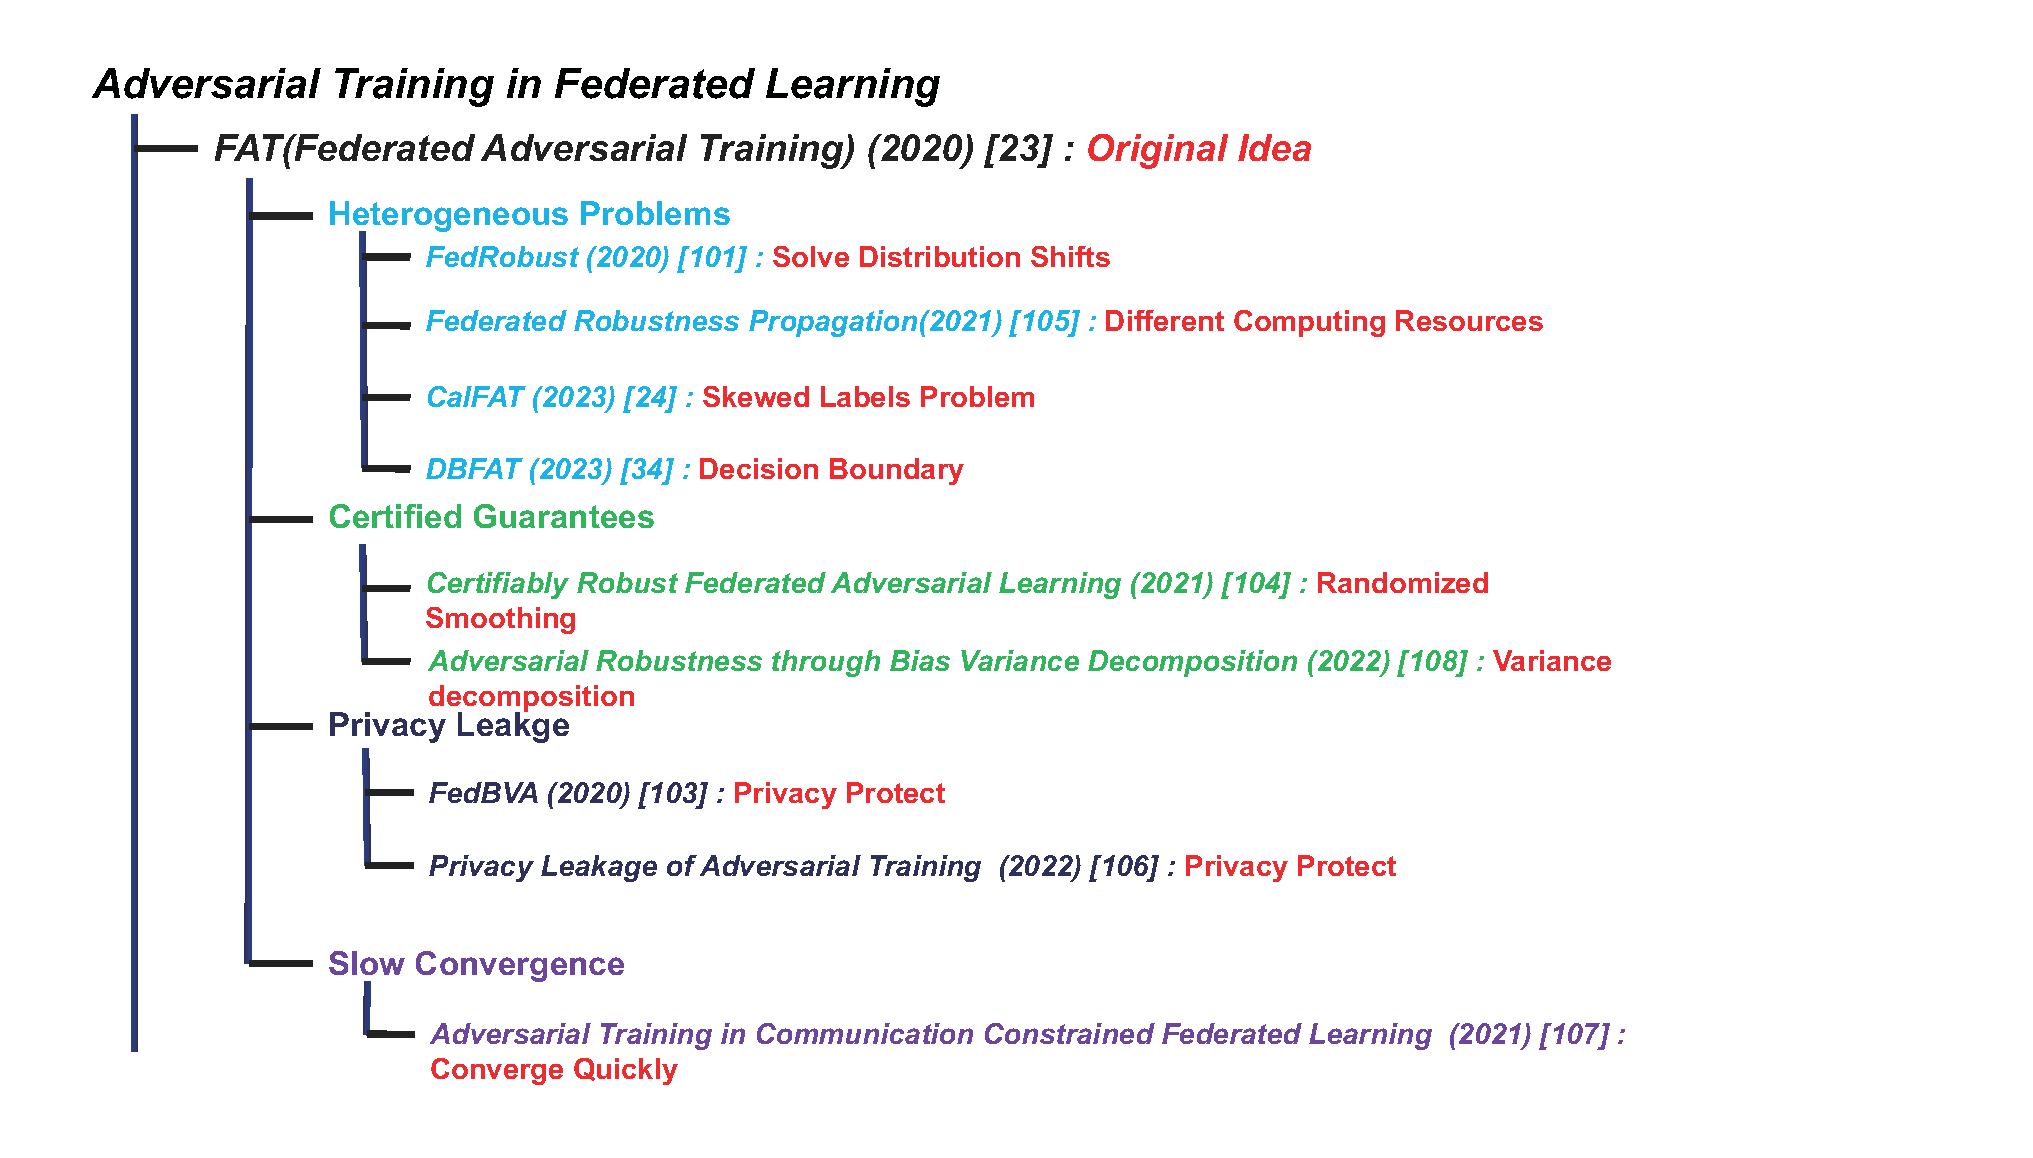
\includegraphics[width=1.0\linewidth,height=2.5in]{output/fig20.eps}
     \caption{}
     \label{fig20}
\end{figure*}


So, there are also several challenges with
implementing adversarial training in federated learning, such as
heterogeneous clients caused by distribution, certified
guarantees, privacy leakage, and slow convergence rate.

\section{Heterogeneous Clients Caused by Distribution}  
The major challenge in federated learning is the
heterogeneity of clients. This means that the distribution of
training data may vary among different clients, and the
computational resources available to each client may also
differ. The paper [101] proposes a novel method called
FedRobust to address the problem of distribution shifts
in federated learning. FedRobust is a gradient descent
ascent (GDA) algorithm that solves the minimax robust
optimization problem and can be efficiently implemented
in a federated setting. This paper shows that FedRobust,
which alternates between the perturbation and parameter
model variables, will converge to a stationary point in the
minimax objective that satisfies the Polyak-Łojasiewicz
(PL) [102] condition. This optimization method can be
used to address the issue of distribution shifts in federated
learning, which can significantly impact the performance
of the trained model. 

\begin{figure}[h]
    \centering
    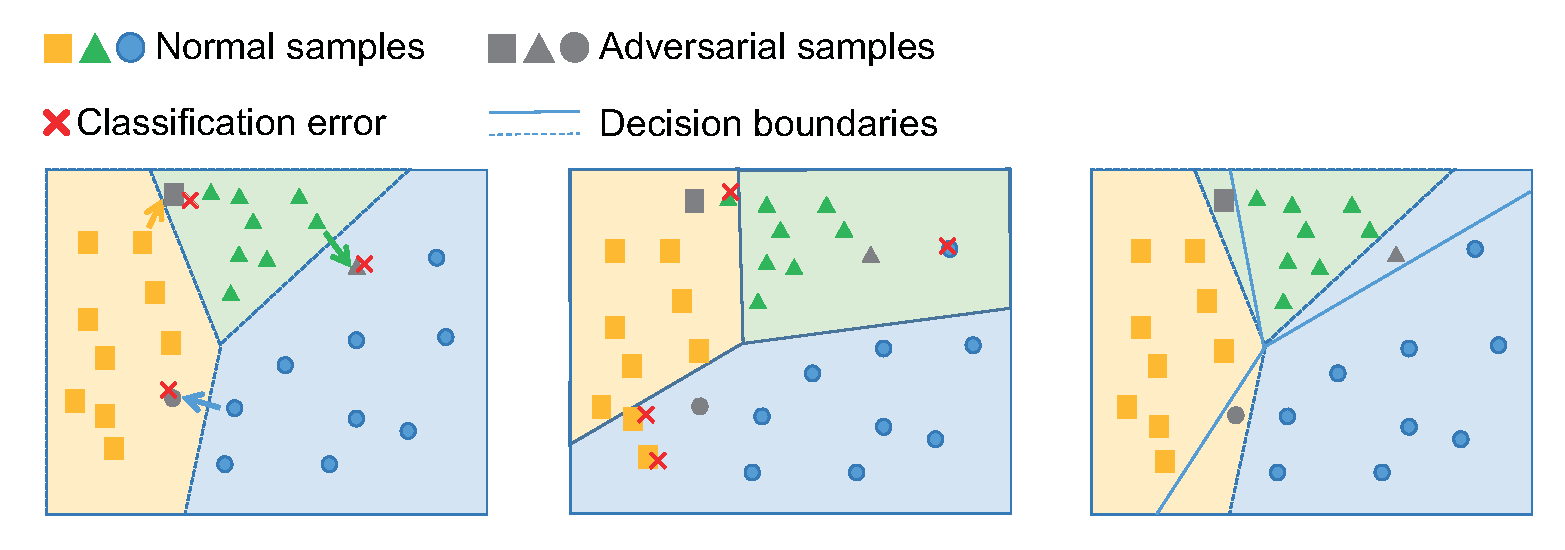
\includegraphics[width=1.0\linewidth,height=2.5in]{output/fig21.eps}
     \caption{}
     \label{fig21}
\end{figure}


Zhang et al. [34] find that the accuracy of the federated
learning model with adversarial training decreases on
clean data, especially when the data of different clients
are non-independent and identically distributed, so they
propose an algorithm based on decision boundary as
shown in Fig.21, which uses local reweighting and global
regularization to improve the accuracy and robustness in
federated adversarial training. Chen et al. [24] study the
skewed labels problem in federated learning and proposes
a CalFAT framework to calculate the logits of each class.
By using this framework, the models between different
clients eventually converge, enhancing the robustness and
accuracy of the global model.
Hong et al. [105] have studied the problems caused
by clients with different computing resources. During
federated learning, some clients can support adversarial
training, but some clients with lack of computing resources
can not support it. This paper studies how to spread
resistance robustness from resource-rich users who can
support confrontation training to those users with poor
resources. This paper shows that an effective robust
propagation algorithm is proposed by using BN layer
technology correctly.

\subsection{Certified Guarantees}  
Certified guarantees are needed in adversarial training
to ensure reliable protection and security against unknown
attacks in adversarial environments. Certified guarantees
refer to rigorous proofs and assurances of model
performance. They provide protection bounds against specific
types of attacks, indicating that the model can maintain
a certain level of performance regardless of how carefully
the attacker designs the attack, such as high accuracy or
robustness.

By using certified guarantees, adversarial training can
provide a degree of predictability and security. This means
that in practical deployment, there is higher confidence in
the model's performance and trustworthiness, rather than
relying solely on trial-and-error evaluation and protection.
It offers a more reliable and definitive defense mechanism
for models to handle unknown or complex attacks.
Chen et al. [104] propose incorporating randomized
smoothing techniques into federated adversarial training
to enable data-private distributed learning with
certifiable robustness to test-time adversarial perturbations.
The experiments conducted in the paper show that this
approach can deliver models as robust as those trained
by centralized training, and can enable provably-robust
classifiers to 2-bounded adversarial perturbations in a
distributed setup.

From the perspective of variance-bias decomposition,
Zhou et al. [108] decompose the loss function into a
combination of bias and variance, generate adversarial
samples on the server and return them to each client for
adversarial training. Then, they used any model
aggregation algorithm to improve the global model's adversarial robustness.  

\subsection{Privacy Leakage}  
As mentioned earlier, privacy protection is crucial in
federated learning. In [106],it is proved that the model of
confrontation training is more prone to privacy disclosure
than the model of normal training. Zhou et al. [103]
argue that conventional federated learning frameworks are
vulnerable to strong adversarial attacks, even if adversarial
training using locally generated adversarial examples is
performed on each client. To address this problem, the
paper proposes a new framework called FedBVA (Federated
Learning with Bias-Variance Analysis) that provides a tiny
amount of bias-variance perturbed data from the central
server to the clients through asymmetrical communication.
This approach dramatically improves the robustness of the 
training model under various settings, without violating
the clients' privacy.

\subsection{Slow Convergence Rate}

As described in [34], conducting adversarial training
in federated learning is a challenging task because the
convergence speed of adversarial training is very slow.
In [107], a method is proposed to solve this problem.
Assuming the local iteration number of federated learning
is E, this article believes that a larger E will increase the
drift between models and affect the adversarial robustness,
but will converge quickly. A smaller E will increase
the adversarial robustness but decrease the convergence
efficiency. Therefore, this article proposes a dynamic
mechanism for adjusting E, and uses FedCurv instead of
FedAvg as the global aggregation algorithm, and proposes
a new algorithm called FedDynAT to simultaneously
improve the convergence speed and adversarial robustness.
As shown in table III, we list some of the methods
mentioned above for comparison. It can be seen from the
table that the adversarial robustness in federated learning
is still weak (less than 40\%). Therefore, the study of
adversarial training in federated learning is still a very
urgent matter. 

\begin{table}[t]
    \caption{\textbf{Comparison of FAT}}
    \label{Comparison of FAT}
    \centering
    \begin{tabular}{|c|c|c|c|} % 有七列,使用 "c" 表示居中对齐,没有竖线
    \toprule % 第一道横线
    \textbf{Paper}  & \textbf{Accuracy} & \textbf{Robustness}\\ 
    \midrule
     MixFAT& $53.35\%$ &   $29.14\%$ \\
     \midrule
     FedRBN& $47.80\%$ &  $26.87\%$ \\
     \midrule
     CalFAT& $64.69\%$ & $35.03\%$   \\
     \midrule
     DBFAT& $52.16\%$ &  $27.80\%$  \\
     \midrule
     FedBVA& $83.8\%$ &  $21\%$  \\
     \midrule
     FedPGD& $46.96\%$ &  $28.7\%$  \\
     \midrule
     FedAvg& $80.5\%$ &  $9.9\%$  \\
    \toprule
    % 继续插入更多数据行
    \end{tabular}
    \end{table} 